% !TEX root = ../../../main.tex
% 来源：中学数学实验教材·第三册（高中数学）
% 章节：三角函数的图象和性质 / 正弦函数的图象和性质
% 原始文件：7.tex，行 72-103
% 类型：tikz
% ---
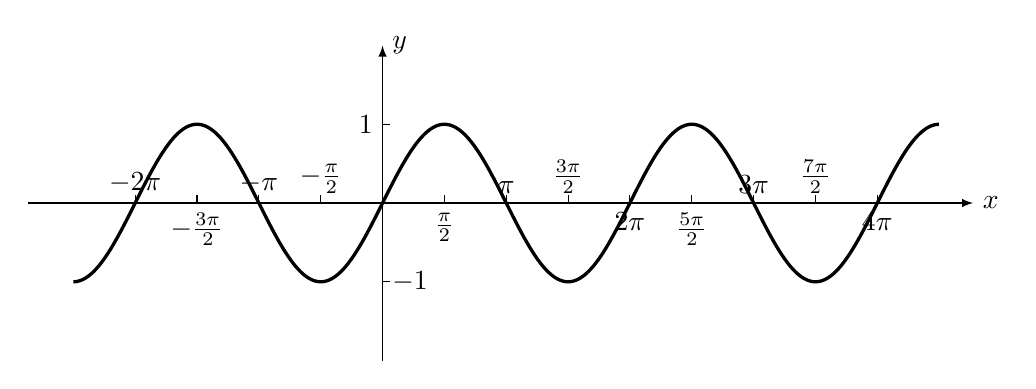
\begin{tikzpicture}[>=latex, xscale=.5]
\draw[->](-9,0)--(15,0)node[right]{$x$}; 
\draw [->](0,-2)--(0,2)node[right]{$y$};
    
\draw[domain=-2.5*pi : pi*4.5,  samples=2000, very thick] plot(\x, {sin(\x r)});

\foreach \x in {-4,-3,...,8}
{
    \draw (\x/2*pi,0)--(\x/2*pi,0.1);
}
\node at (-2*pi,0)[above]{$-2\pi$};
\node at (-1.5*pi,0)[below]{$-\frac{3\pi}{2}$};
\node at (-1*pi,0)[above]{$-\pi$};
\node at (-.5*pi,0)[above]{$-\frac{\pi}{2}$};
\node at (.5*pi,0)[below]{$\frac{\pi}{2}$};
\node at (1*pi,0)[above]{$\pi$};
\node at (1.5*pi,0)[above]{$\frac{3\pi}{2}$};
\node at (2*pi,0)[below]{${2\pi}$};
\node at (2.5*pi,0)[below]{$\frac{5\pi}{2}$};    
\node at (3*pi,0)[above]{$3\pi$};
\node at (3.5*pi,0)[above]{$\frac{7\pi}{2}$};
\node at (4*pi,0)[below]{$4\pi$};


\draw (0,1)--(.2,1);
\draw (0,-1)--(.2,-1);
\node at (0,1)[left]{1};
\node at (0,-1)[right]{$-1$};



\end{tikzpicture}
